%\documentclass[twocolumn,english,aps,preprint,prl,reprint,superscriptaddress,longbibliography]{revtex4-1}
%\begin{document}

\vspace{-0.5em}
\centering{{\noindent \large \textbf{Growth and preservation of entanglement in a many-body localized system}}}
\vspace{1.0em}

\setcounter{topnumber}{2} %  maximum number of floats in the top area
\setcounter{bottomnumber}{2} % maximum number of floats in the bottom area
\setcounter{totalnumber}{4} % maximum number of floats on a text page
\renewcommand{\topfraction}{0.99} % The maximum size of the top area
\renewcommand{\bottomfraction}{0.99} %The maximum size of the bottom area
\renewcommand{\textfraction}{0} %  The area that must not be occupied by floats
\renewcommand{\floatpagefraction}{0.999} % the minimum part of the page that need to be occupied by floats to for a float page
\setlength{\floatsep}{5pt plus 2pt minus 2pt}  % The separation between floats in the top and bottom areas
\setlength{\textfloatsep}{5pt plus 2pt minus 2pt} % The separation between the top or bottom area and the text area
\setlength{\intextsep}{5pt plus 2pt minus 2pt}  % For inline floats (placed by "here")

%\setlength{\abovedisplayskip}{1pt}
%\setlength{\belowdisplayskip}{1pt}

\begin{abstract}
\textbf{In non-interacting systems disorder leads to Anderson localization, where particle diffusion and entanglement propagation are absent.
Interactions between the constituent particles modify this picture, leading to a many-body localized (MBL) phase.
A key challenge is to measure interaction induced dynamics of entanglement between the localized sites in this phase.
By studying interacting photons in an array of superconducting qubits, we observe ergodicity breaking and directly measure the effective non-local interactions.
We probe the entanglement signatures of MBL in 1D and 2D and observe the slow growth of entanglement entropy.
Finally, we characterize the potential of the MBL phase to be used as a “quantum memory” by demonstrating the slow decay of entanglement of a distant bell pair.
Our work elucidates the fundamental mechanisms of entanglement formation, propagation, and preservation in the MBL phase of matter. }
\end{abstract}

\maketitle

\section{} % Introduction
\vspace{-14mm}

Disorder-induced localization is a ubiquitous phenomenon that occurs in both classical and quantum systems. In 1958 Anderson showed that in non-interacting systems disorder can change the structure of electronic wave-functions from being extended to exponentially localized\,\cite{Anderson1958}. This localized phase has been observed for systems of non-interacting phonons, photons, and matter-waves\,\cite{The50years,Billy2008, Weaver1990, Wiersma1997, Schwartz2007}.  The conventional wisdom had long been that systems of interacting particles do not localize and ultimately reach thermal equilibrium regardless of the disorder magnitude. However, recent work suggests that localization may persist even with the introduction of interactions between particles, thus establishing the concept of many-body localization as a robust, non-ergodic phase of matter at finite temperature\,\cite{Basko2006, Gornyi2005, ImbriePRL2016}.

\begin{figure}[h!] % figure 1
\centering
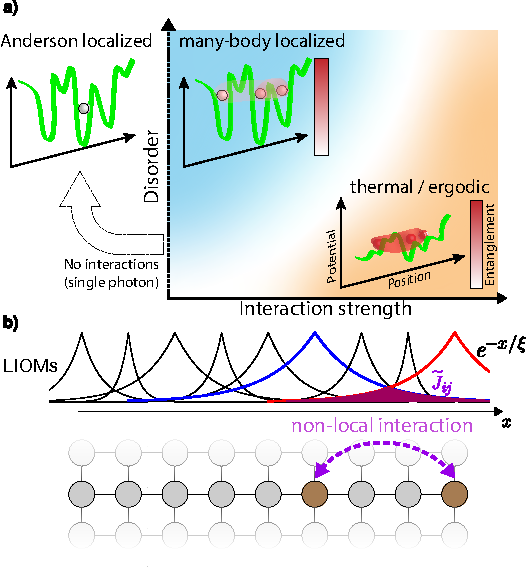
\includegraphics[width=75mm]{./PDF/fig_1.pdf}
\vspace{-0.7em}
\caption{ \textbf{Many-body localization with superconducting qubits.} \textbf{(a)} In 1D, Anderson localization occurs for arbitrarily weak disorder potentials. Interactions between the particles facilitate delocalization and entanglement propagation. When disorder is large, the MBL phase is realized and the particles remain localized but entanglement spreads. As the interactions are increased, the system transitions to a thermalized phase with fully delocalized and entangled particles. \textbf{(b)} The localized orbitals (local integrals of motion, LIOM) decay exponentially in space with a broad distribution of localization lengths $\xi$ and couplings $\widetilde{J}_{ij}$ between them. The shaded region indicates effective non-local interactions between two LIOMs.}
\end{figure}
% \afterpage{\FloatBarrier}

\begin{figure*}[t] %figure 2
\centering
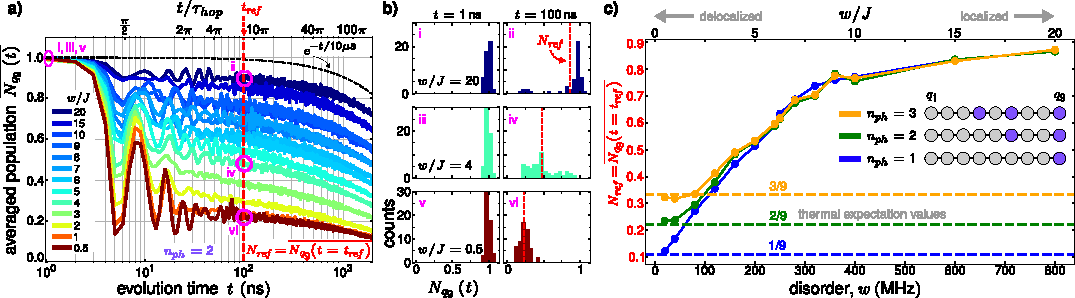
\includegraphics[width=178mm]{./PDF/fig_2.pdf}
\vspace{-0.7em}
\caption{\small
\textbf{Ergodicity breakdown.} \textbf{(a)} Disorder averaged on-site population vs. time for $n_{ph}=2$. In a chain of 9 qubits, two qubits were excited ('q6', 'q9'). The on-site population of 'q9' was measured with resolution of $\ket{0}$, $\ket{1}$, $\ket{2}$ for various magnitudes of disorder $w/J$, with $J=40\,\text{MHz}$. The overline indicates average over disorder realizations, and each data point is the average of 50 realizations. The parameter $\tau_{hop}=\left(2 \pi J \right)^{-1}$ has been introduced to connect the laboratory time $t$ with the hopping energy. $N_{ref}$ is defined to be the average on-site population across instances of disorder at the reference time $t_{ref}=100\,\text{ns}$, after initial transients have been damped. The dashed black line indicates expected photon loss for a single qubit measured in isolation. \textbf{(b)} Histograms of $\nqninet$  at the times and disorders indicated in \textbf{(a)} by numerals i - vi. \textbf{(c)} $N_{ref}$ vs. disorder for $n_{ph}=1, 2, 3$. Inset shows which qubits were excited at $t=0$ ns.}
\vspace{-1em}
\end{figure*}

Various experimental studies show that some characteristics of the MBL phase resemble a conventional non-interacting Anderson phase in which relaxation is absent\,\cite{BlochMBL2015, demarco2015, Monroe2015, GrossScience2016, Bordia2017, Roushan2018, Lukin2019}; both Anderson localized and MBL phases do not thermalize. Theoretical studies suggest that the MBL phase has significantly different dynamical properties\,\cite{Huse2007, Bardarson2012, Serbyn2013b, Huse2014, Serbyn2013, KnapPRL2014, Antonello2017, Serbyn2014, Yasaman2015,  Gopalakrishnan2015, Serbyn2015, Altman2015, ImbriePRL2016}. In particular, resulting from the non-local interaction between particles it is anticipated that locally observed dephasing arises during the coherent closed-system dynamics\,(Fig.\,1). It has been predicted that this dephasing leads to the slow growth of entanglement entropy in the MBL phase. The direct study of this physics is experimentally challenging as it is best accomplished with phase sensitive algorithms and measurement. Superconducting qubit systems allow a comprehensive study of interaction effects in the MBL phase, since they offer capabilities to perform versatile wave function initialization, Hamiltonian generation, and measurements in different bases.

Using an array of superconducting qubits, we realize a bosonic lattice and study the dynamics of photon excitations as a function of disorder. The Hamiltonian of the chain is described by the Bose-Hubbard model
%\vspace{-10pt}
\begin{eqnarray}
H_{BH} &=& \underbrace{\sum\limits_{i}^{n_Q} h_i a^{\dagger}_{i}a_{i}}_{\text{on-site detuning}} +
\underbrace{\frac{U}{2}\sum\limits_{i}^{n_Q} \,a^{\dagger}_{i}a_i(a^{\dagger}_{i}a_i-1)}_{\text{Hubbard interaction}} \nonumber \\
&+& \underbrace{J \sum_{\left< i, j \right>}\left( a^{\dagger}_{i}a_j+a_{i}a^{\dagger}_{j} \right) }_{\text{NN coupling / hopping}},
\end{eqnarray}
%\vspace{-10pt}
\noindent
where $a^{\dagger}$ ($a$) denotes the bosonic creation (annihilation) operator, $h_i\in \left[ -w, w \right]$ is the random on-site detuning drawn from a uniform distribution of width $2w$, $J$ is the hopping rate between nearest neighbour lattice sites, $U$ is the on-site Hubbard interaction, and $n_Q$ is the number of qubits\,\cite{supplement}. The qubit frequency, the nearest neighbor coupling, and nonlinearity set $h_i$, $J$, and $U$, respectively. We are able to tune the $h_i$ and $J$ independently at a fixed nonlinearity $U=160$ MHz.

The localized regime of Eqn.\,(1) is obtained when the frequency detunings $h_i$ are large compared to $J$. In this regime, the eigenstates of the Hamiltonian are product states of localized orbitals, referred to as local integrals of motion (LIOM), which are nearly qubit states but have a spatial extent that decays exponentially across the neighboring qubits\,(Fig.\,1(b)). In the localized regime, Eqn.\,(1) can be brought into a diagonal form by a set of local unitary transformations\,\cite{Serbyn2013, Huse2014}. In this basis there is no hopping and the Hamiltonian can be written in terms of on-site detunings and non-local interactions,
\vspace{10pt}
\begin{equation} % tau Hamiltonian
\tilde{H}_{\tau} = \underbrace{\sum_i \widetilde{h}_i \tau^z_i}_{\text{on-site detuning}} + \underbrace{ \sum_{i,j} \widetilde{J}_{ij}\tau^z_i\tau^z_j + \sum_{ijk} \widetilde{J}_{ijk}\tau^z_i\tau^z_j\tau^z_k + \mathellipsis.}_{\text{non-local interaction}}% = \sum_i \delta_i \left( \tau^z_{j \neq i}\tau^z_i \right).
\end{equation}
\noindent
The $\tau^z_j$ operators commute with $\tilde H_{\tau}$ and are hence conserved; the system is localized. However, the non-local interactions $\widetilde{J}$, which follow a broad log-normal distribution, generate entanglement throughout the localized system\,\cite{Varma2019}.

\section{} % Ergodic breakdown
\vspace{-16mm}

\textcolor{blue}{ Evidence for the breakdown of ergodic dynamics} can be obtained by measuring the mobility of excitations in a 1x9 qubit array. In Fig.\,2, we initialize the system with a number of photon excitations $n_{ph}$ by preparing $1$, $2$, or $3$ qubits in the single excitation Fock state. We measure the population on one of the initially excited qubits as the system evolves under Hamiltonian\,(1).

The disorder averaged population at $q_9$ (the observation site) $\overline{ \nqninet }$ for $n_{ph}=2$ is shown in panel (a). We choose a reference time $t_{ref}$, in which $\overline{ \nqninet }$ approaches an asymptotic value after initial transients have been damped, before the dynamics of our system are dominated by relaxation to the environment at large time scales (dashed black line), or delocalization within our closed system driven by extrinsic dephasing\,\cite{supplement,Znidaric2015, Levi2016, Fischer2016, Luschen2017, vanNieuwenburg2017}. The distribution of $\nqninet$ for selected disorder magnitudes at $t=1\,\text{ns}$ and $t=t_{ref}$ are shown in panel (b). At $t=1\,\text{ns}$ the excitations have not propagated, and there is a tight distribution close to the initial values, regardless of the value of disorder. At $t=t_{ref}$ the distribution is narrow for low disorder and becomes wider with tails at larger disorders. This can be understood because at high disorder, level resonances are increasingly rare which inhibits mobility. The tail of the distribution results from these rare cases. At low disorder, excitations can propagate freely between qubits and the behavior of each disorder instance is typical, giving rise to narrow distributions.

\begin{figure}[t]
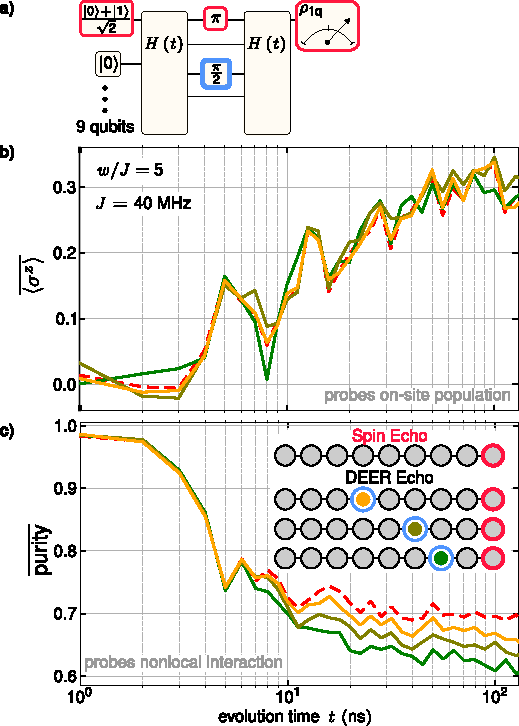
\includegraphics[width=70mm]{./PDF/fig_3.pdf}
\vspace{-0.7em}
\caption{\small
\textbf{Interferometric signatures of remote entanglement.}
\textbf{(a)} SE and DEER pulse sequences. DEER differs from SE by the addition of a remote $\pi\, /\,2$-pulse simultaneous with the SE $\pi$-pulse between the free precession intervals. \textbf{(b)}  $\overline{ \left< \sigma^z \right> } =\overline{ \left< 1 - 2 a^\dagger a \right> }$, and \textbf{(c)}  purity of the single qubit for SE (red dashed) and DEER (solid) experiments. The remote DEER pulse induces dephasing, decreasing the purity. The contrast between SE and DEER probes the non-local interaction $\widetilde{J}_{ij}$ between the SE lattice site and the DEER site.}
\end{figure}

Fig.\,2(c) shows the disorder averaged population after $t_{ref}=100\, \text{ns}$ of evolution as a function of the disorder strength. At low disorder, in the diffusive regime, we expect the dynamics to satisfy the ergodic hypothesis that each of the two photon states is equally likely to be observed. Here, a uniform averaging over the available phase space implies that the expected occupancy of a given qubit should be $n_{ph}\,/n_Q$. For multiple photon excitations our observations are consistent with ergodic dynamics at weak disorder; however, as we increase the disorder strength, significant deviations from the thermal value are observed, which indicates that our system becomes many-body localized. We note that with more photons in the system, the population converges to its thermal expectation value at higher disorders. This is expected because the increased interactions assist with the thermalization process and drive delocalization. In the case of a single excitation our system is non-interacting and hence localized for all disorder magnitudes. The apparent approach of the population to the thermal value at extremely weak disorder indicates the regime where the single-particle localization length exceeds our system size.  The ergodicity breaking shown here is general and the results for the 2D system can be found in the supplement\, \cite{supplement}.
\section{} % Interferometric methods
\vspace{-16mm}

\textcolor{blue}{Nonlocal interactions between the LIOMs} can be unambiguously established by adopting interferometric methods inspired by NMR protocols\,\cite{KnapPRL2014}.  Fig.\,3(a) illustrates a conventional spin-echo (SE) sequence and its extension double electron-electron resonance echo (DEER) which we use to provide a differential measurement of phase accumulation with and without a remote perturbation. The construction and effects of these pulse sequences can be understood from Eqn.\,(2). Deep in the MBL phase, the LIOMs are nearly localized on individual qubits. The SE $\pi$-pulse between free precession intervals essentially negates the local frequency detuning, reversing the evolution and hence phase accumulation. The role of the additional $\pi/2$-pulse in the DEER sequence is to make the SE refocusing incomplete, directly probing the strength of the non-local interaction. The measurement of on-site population, depicted in panel (b), shows that the remote $\pi / 2$-pulse in the DEER sequence does not appreciably alter the population on the observation site, assuring that the system is in the localized regime. Therefore, comparing SE and DEER, the contrast observed in the single qubit purity\,(panel (c)), is a pure interference effect that directly measures the non-local interaction between distant localized sites. In addition, the difference between SE and DEER decreases as the distance between the SE site and remote disturbance site is increased. This can be understood from the decaying nature of the interactions between the LIOMs with distance. The interferometric protocol is thus demonstrating the foundational interaction effects of MBL states.


\begin{figure}[t]
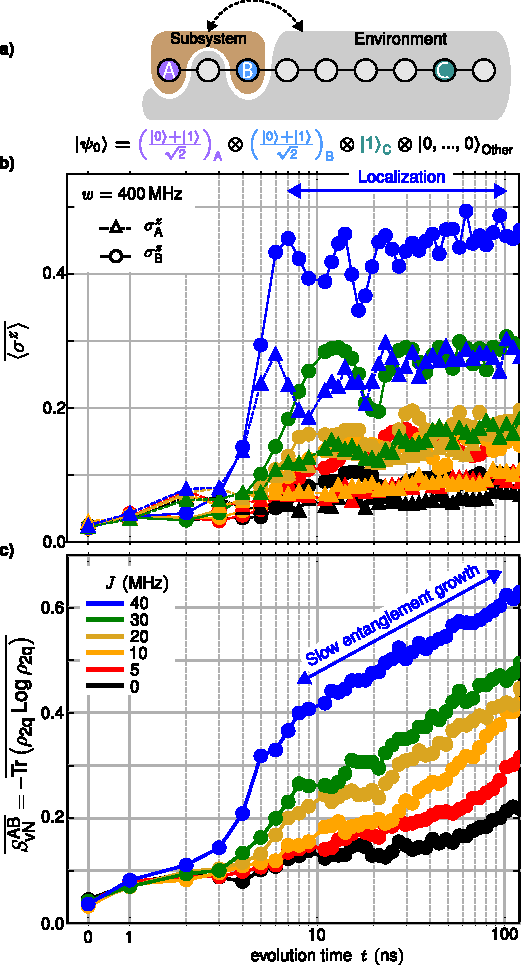
\includegraphics[width=70mm]{./PDF/fig_4.pdf}
\vspace{-0.7em}
\caption{\small{
\textbf{Localization and slow growth of entanglement}
\textbf{(a)} Partitioning of our 9-qubit chain into a subsystem and environment.
 The subsystem qubits (A and B) are initialized into superposition states, and the system is loaded with an additional excitation (site C) to enhance many-body interactions. We tomographically reconstruct the  density matrix of the subsystem. \textbf{(b)} $\overline{\left< \sigma^z \right>}$ for subsystem qubits. \textbf{(c)} von Neumann entanglement entropy of the two qubit subsystem for several coupling strengths.}}
\end{figure}


\textcolor{blue}{A hallmark of the MBL phase} is the slow growth of entanglement, contrasting with Anderson localization where the entanglement is constant. To study the development of entanglement entropy, we designate two qubits as a subsystem and the rest of the chain as the environment (Fig.\,4(a)), and directly measure the evolution of the reduced density matrix of the subsystem. The subsystem qubits are initialized into superposition states. Fig.\,4(b) shows that $\overline{ \left< \sigma^z \right> }$ initially rises because population from the subsystem qubits is transferred to the environment which has a smaller photon density. After this initial rise, $\overline{ \left< \sigma^z \right> }$ takes a stationary value which decreases with decreasing coupling strength, establishing the localization of our system.

We use the von Neumann entanglement entropy
\begin{equation}
S_{\text{vN}}=-\text{Tr} \rho_{\text{2q}} \text{log} \rho_{\text{2q}}
\end{equation}
\noindent to quantify the entanglement between the subsystem and the environment (panel\,(c)).
The initial increase in $\overline{ S_{\text{vN}} }$ occurring simultaneously with the increase in $\overline{ \left< \sigma^z \right> }$ is understood as the result of the subsystem exchanging population with the environment.  Thereafter, while the system is demonstrably localized, we observe logarithmic growth of von Neumann entropy. We can understand the slow growth in terms of the LIOM framework: The non-local and exponentially decaying interactions between the LIOMs give rise to dephasing between the qubits and follow a broad log-normal distribution\,\cite{Varma2019}. As a consequence, the entanglement of individual runs is strongly fluctuating on different time scales leading to a logarithmic growth of the entanglement of the subsystem. We note that preparing subsystem qubits in an x-polarized state is key for the success of this measurement as it enhances the measurement visibility by being highly phase sensitive. The von Neumann entropy quantifies entanglement with all external degrees of freedom and is not able to disambiguate entanglement with the environmental qubits due to unitary dynamics from open systems effects.  As such, our observed entropy is an upper bound on the entanglement generated within our qubit array.  The $J=0$ curve (black) provides an estimate of the amount of entropy that is due to open system effects.  Next, we introduce entanglement measures that are more robust against open systems effects and lower bound the entanglement between parts of the system.

\section{} % growth and preservation

\vspace{-14mm}

\begin{figure*}[t] % Figure 5
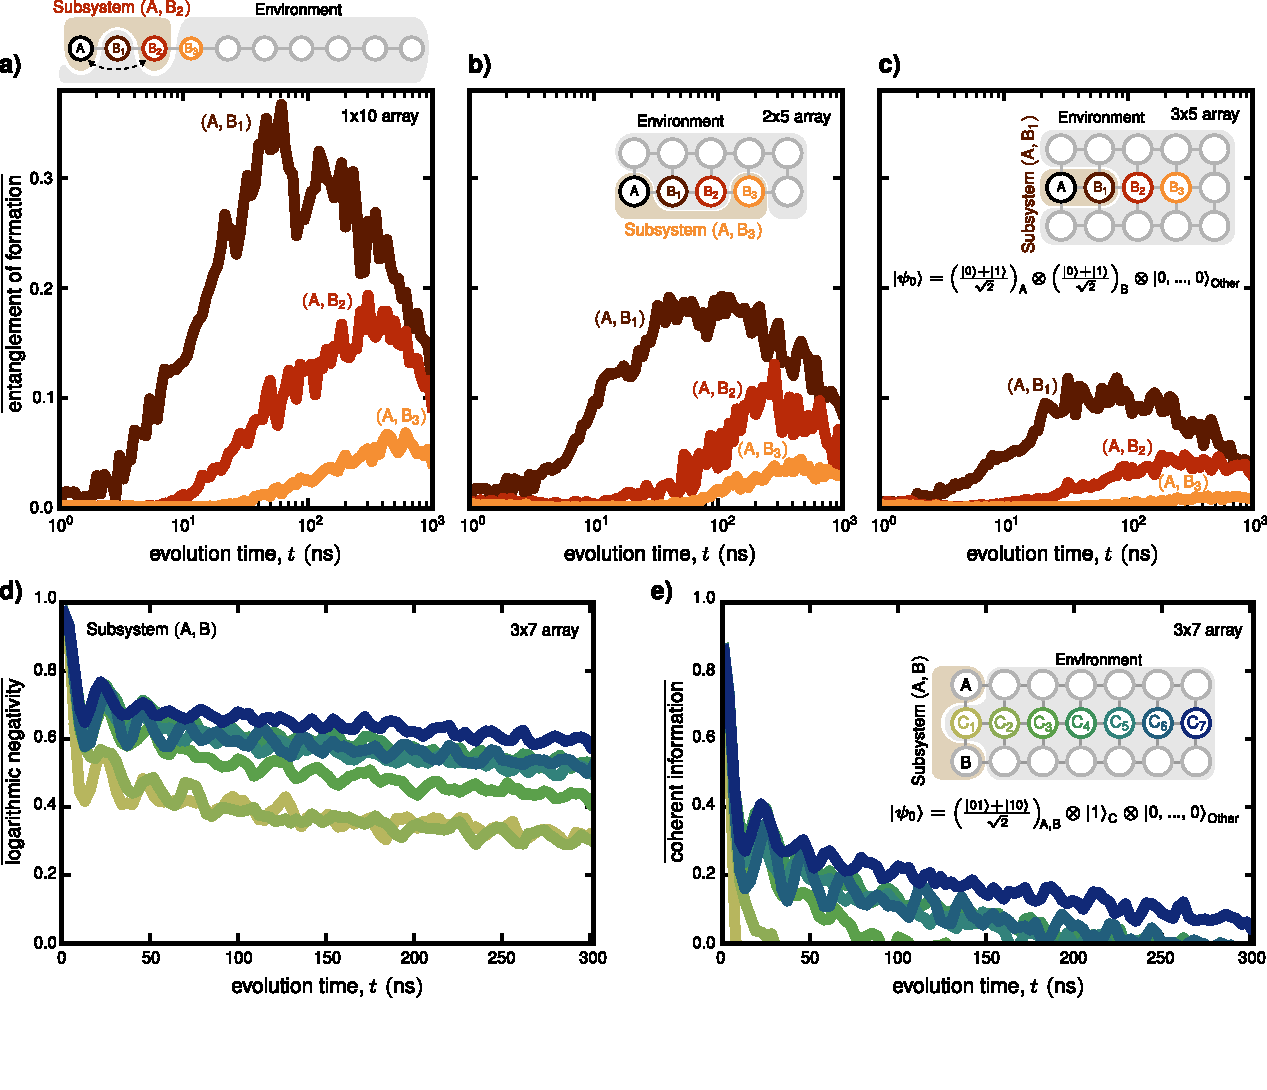
\includegraphics[width=160mm]{./PDF/fig_5.pdf}
\vspace{-4.5em}
\caption{\small \textbf{Growth and preservation of entanglement between localized sites}
Entanglement of formation between qubits in various 2-qubit subsystems (A,B$_i$). To observe the development of entanglement between sites A and B the subsystem is initialized in a product of single qubit superposition states and the entanglement of formation of the two qubit density matrix is extracted, for subsystems of \textbf{(a)} $1\times10$, \textbf{(b)} $2\times5$, and \textbf{(c)} $3\times5$ array of qubits with $J=30$\,MHz and $w/J=10$. In a 2 qubit subsystem (A,B) of a 3 by 7 array of qubits, a Bell pair is created, and the Logarithmic negativity \textbf{(d)} and coherent information \textbf{(e)} are extracted from measurements of the subsystem density matrix and averaged over 80 realizations of disorder for $J=30$\,MHz with $w/J=12$.  We initialize the environment with an excitation at a position $C_i$ which is varied}
\end{figure*}

%Schematic diagram emphasizing our focus on the entanglement between qubits A and B$_i$ which are embedded in an environment.


\textcolor{blue}{We investigate the formation and preservation of entanglement} between two qubits A and B that are embedded in a MBL environment as illustrated in Fig.\,5(a). The entanglement of formation (EOF) quantifies the amount of entanglement directly between qubits A and B that would be required to produce the observed two-qubit mixed state density matrix\,\cite{Wootters1998}.   This entanglement can be viewed as the elemental building block of the $S_{\text{vN}}$ in Fig.\,4. We emphasize that because we are affirmatively detecting a quantum correlation between sites of the subsystem, the observed EOF cannot be attributed to open system effects which would tend to suppress the correlation.  The EOF is therefore a more conservative entanglement measure than $S_{\text{vN}}$ and a valuable tool for characterizing realistic experimental systems, which are semi-open.

In (a) to (c), we initialize the subsystem in a product state of single qubit superpositions and observe the development of entanglement between the subsystem qubits. Regardless of geometry of the qubit array, entanglement grows gradually between the localized, spatially separated sites over several hopping times.  Intuitively, the entanglement grows faster and achieves a higher maximum value when the subsystem qubits are closer to each other. This can be understood by considering two isolated qubits, which exhibit a cosine shaped growth and collapse of their mutual entanglement at a frequency that is set by the effective interactions $\widetilde{J}_{ij}$, explaining the shift of the first maximum toward much larger times as the distance is increased. Due to the presence of the other qubits in our system, the entanglement deviates from the cosine shape after the first maximum\,\cite{Serbyn2013b}.  At long times open systems effects become important. The EOF results are in contrast to the von Neumann entropy, which continuously increases because it includes entanglement with all degrees of freedom external to the subsystem.

As the system geometry is transformed from 1D into a ladder and finally 2D (panels (a) to (c)) there is an overall trend of suppressed EOF.  This can be understood by considering the mobility in combination with the monogamy of entanglement principle\,\cite{Wootters2000}. Compared with 1D, in 2D each qubit has additional neighbors, which changes the structure of the LIOMs and provides more transport channels, enhancing the spread of entanglement.  The monogamic principle states that there is a maximum degree to which two qubits may be correlated, and that entangling (correlating) either member of this pair with other qubits necessarily decorrelates the first two.  Thus in the higher dimensional systems shown here the subsystem qubits entangle with the environmental qubits to a greater extent thereby reducing the degree to which the subsystem qubits can be correlated.

At long times, the interaction between subsystem qubits is out competed by the interaction of the subsystem with the environmental qubits and the open system and the EOF declines.  We highlight the capability of EOF, an affirmative correlation measure, to detect correlation between sites with large separation, e.g. (A, B$_3$) despite being embedded in a large entangled array with open system effects.


The results thus far illustrate how interaction effects propagate entanglement throughout the system.  However, because MBL systems are non-thermal and localized, features of their initial state remain imprinted on them.  This ability of MBL systems to retain quantum correlations as a computational resource for later retrieval suggests their potential as a quantum memory \cite{Huse2014, Moore2015, Cirac2017}.  To probe this aspect, we prepare a maximally entangeled Bell state between two subsystem qubits in a 3$\times$7 qubit array and monitor the subsystem density matrix as the pair is dephased by a remote photon. %Dephasing between LIOMs will ultimately destroy the entanglement, but only at exponentially long times.
%We therefore characterize the entanglement of the 2-body mixed density matrix $\rho_{2q} \left( t \right)$ using an operational entanglement measure.
We focus on the distillable entanglement (DE), i.e. the entanglement which can be extracted from the mixed density matrix.  The upper and lower bounds of the DE are the logarithmic negativity entropy and the coherent information entropy respectively, shown in Fig. 5\,(d) and (e).

The initial drop of DE, on the single hopping timescale, is attributed to population transfer from the Bell pair into the environmental qubits. Thereafter, interaction with the remote photon induces local dephasing in the subsystem, decorrelating the subsystem qubits according to the monogamy of entanglement principle.  With the remote photon at larger distances, the DE remains finite over several hopping times.  The entanglement is increasingly disturbed as the remote photon is brought closer to the Bell pair and the coherent information that lower bounds the DE approaches zero at earlier times.  This data illustrates the potential of the MBL phase as a quantum memory and highlights excitation density as a critical parameter for this application.

\vspace{1em}

\begin{comment}
While the results discussed thus far show interaction effects between the LIOMs, it is also a major prospect to demonstrate the preservation of quantum information in such a system. To this end, we prepare a distant maximally entangeled Bell state between two qubits located in the first and third row of a 3$\times$7 array of qubits and study the entanglement dynamics. While dephasing between LIOMs will ultimately destroy the entanglement, it will only due so on exponentially long times. Crucially, the subsystem is in a mixed state because of its coupling to the other environment qubits. We therefore characterize the entanglement of the 2-body mixed density matrix $\rho_{2q} \left( t \right)$ using an operational entanglement measure. In particular, we focus on the distillable entanglement, i.e., the entanglement which can be extracted from the mixed density matrix, that is upper bounded by logarithmic negativity entropy (panel\,(d)) and lower bounded by the coherent information entropy (panel\,(e)).

To probe the stability of the Bell pair and measure the degree of its preservation, we initially added another photon to the environment at different positions. The initial sudden drops of entanglement measures are due to quench, where the excitations fill out the LIOMs in the one hopping time scale. The overall decay of the entanglement is the characteristic MBL dephasing, which shows sensitivity to the position of the other excitation. The extra photon leaves different marks on the two bounds of distillable entanglement, while the logarithmic negativity seems insensitive to the position of extra photon (same slope in panel\,(d)), the coherent information can rapidly destroyed as the photon becomes closer.  Data on panel (d) and (e) illustrates the potential of the MBL phase as a quantum memory and highlights excitation density as a critical parameter for this application.
\end{comment}

%This behavior can also be understood in terms of the monogamy of entanglement\,\cite{Wootters2000}. Although the two qubit subsystem is initially prepared in a maximally entangled state the degree of quantum correlation between subsystem sites decreases as the subsystem exchanges information with the environment and entangles with it. This monogamic principle also explains the damping of the peak in the low disorder data of panel (b). However, for strong disorder (blue) the distillable entanglement is sizable over long times, and hence the density matrix can be used as quantum resource. This is exemplified in panel (d) which shows the evolution of two qubit density matrix for a single disorder instance. These results show that a MBL system can efficiently retain quantum information over long time scales.

\noindent \textbf{Acknowledgments} \footnotesize{ The authors acknowledge valuable conversations with Jens Eisert and Andrew Daley. M.K. and A.B. acknowledge support from the Technical University of Munich - Institute for Advanced Study, funded by the German Excellence Initiative and the European Union FP7 under grant agreement 291763, the Deutsche Forschungsgemeinschaft (DFG, German Research Foundation) under Germany's Excellence Strategy--EXC-2111--390814868, DFG grant No. KN1254/1-1, and DFG TRR80 (Project F8). M.K., A.B., D.A., and M. F. acknowledge support through Google Quantum NISQ award.  M.F. also acknowledges support from the FNS/SNF Ambizione Grant PZ00P2\_174038. S.G. acknowledges support from NSF Grant No. DMR-1653271}

\vspace{1em}
\noindent \textbf{Correspondence and requests for materials}
\small{should be addressed to P. Roushan\,(pedramr@google.com).}

\vspace{1em}
\noindent * These authors contributed equally to this work.

% to do:
% 2) refer to fig S20
%\end{document}


%\author{\small{B. Chiaro$^*$}}
%\affiliation{Department of Physics, University of California, Santa Barbara, California, USA}
%\author{\small{C. Neill$^*$}}
%\affiliation{\footnotesize{Google Inc., Santa Barbara, California, USA}}
%\author{\small{A. Bohrdt$^*$}}
%\affiliation{\footnotesize{Department of Physics and Institute for Advanced Study, Technical University of Munich, Garching, Germany}}
% \affiliation{\footnotesize{Munich Center for Quantum Science and Technology (MCQST), M\"unchen, Germany}}
%\author{\small{M. Filippone$^*$}}
%\affiliation{\footnotesize{Department of Quantum Matter Physics, University of Geneva, Switzerland }}
%\author{\small{K. Arya}}
%\affiliation{\footnotesize{Google Inc., Santa Barbara, California, USA}}
%\author{\small{R. Barends}}
%\affiliation{\footnotesize{Google Inc., Santa Barbara, California, USA}}
%\author{\small{B. Burkett}}
%\affiliation{\footnotesize{Google Inc., Santa Barbara, California, USA}}
%\author{\small{Y. Chen}}
%\affiliation{\footnotesize{Google Inc., Santa Barbara, California, USA}}
%\author{\small{Z. Chen}}
%\affiliation{\footnotesize{Google Inc., Santa Barbara, California, USA}}
%\author{\small{R. Collins}}
%\affiliation{\footnotesize{Google Inc., Santa Barbara, California, USA}}
%\author{\small{A. Dunsworth}}
%\affiliation{\footnotesize{Google Inc., Santa Barbara, California, USA}}
%\author{\small{A. Fowler}}
%\affiliation{\footnotesize{Google Inc., Santa Barbara, California, USA}}
%\author{\small{B. Foxen}}
%\affiliation{\footnotesize{Department of Physics, University of California, Santa Barbara, California, USA}}
%\author{\small{C. Gidney}}
%\affiliation{\footnotesize{Google Inc., Santa Barbara, California, USA}}
%\author{\small{M. Giustina}}
%\affiliation{\footnotesize{Google Inc., Santa Barbara, California, USA}}
%\author{\small{T. Huang}}
%\affiliation{\footnotesize{Google Inc., Santa Barbara, California, USA}}
%\author{\small{E. Jeffrey}}
%\affiliation{\footnotesize{Google Inc., Santa Barbara, California, USA}}
%\author{\small{K. Kechedzhi}}
%\affiliation{\footnotesize{Google Inc., Santa Barbara, California, USA}}
%\author{\small{J. Kelly}}
%\affiliation{\footnotesize{Google Inc., Santa Barbara, California, USA}}
%\author{\small{P. Klimov}}
%\author{\small{F. Kostritsa}}
%\affiliation{\footnotesize{Google Inc., Santa Barbara, California, USA}}
%\author{\small{E. Lucero}}
%\affiliation{\footnotesize{Google Inc., Santa Barbara, California, USA}}
%\author{\small{A. Megrant}}
%\affiliation{\footnotesize{Google Inc., Santa Barbara, California, USA}}
%\author{\small{J. Mutus}}
%\affiliation{\footnotesize{Google Inc., Santa Barbara, California, USA}}
%\author{\small{M. McEwen}}
%\affiliation{\footnotesize{Department of Physics, University of California, Santa Barbara, California, USA}}
%\author{\small{O. Naaman}}
%\affiliation{\footnotesize{Google Inc., Santa Barbara, California, USA}}
%\author{\small{M. Neeley}}
%\affiliation{\footnotesize{Google Inc., Santa Barbara, California, USA}}
%\author{\small{C. Quintana}}
%\affiliation{\footnotesize{Google Inc., Santa Barbara, California, USA}}
%\author{\small{D. Sank}}
%\affiliation{\footnotesize{Google Inc., Santa Barbara, California, USA}}
%\author{\small{K. Satzinger}}
%\affiliation{\footnotesize{Google Inc., Santa Barbara, California, USA}}
%\author{\small{A. Vainsencher}}
%\affiliation{\footnotesize{Google Inc., Santa Barbara, California, USA}}
%\author{\small{T. White}}
%\affiliation{\footnotesize{Google Inc., Santa Barbara, California, USA}}
%\author{\small{P. Yeh}}
%\affiliation{\footnotesize{Google Inc., Santa Barbara, California, USA}}
%\author{\small{A. Zalcman}}
%\affiliation{\footnotesize{Google Inc., Santa Barbara, California, USA}}
%\author{\small{V. Smelyanskiy}}
%\affiliation{\footnotesize{Google Inc., Santa Barbara, California, USA}}
%\author{\small{H. Neven}}
%\affiliation{\footnotesize{Google Inc., Santa Barbara, California, USA}}
%\author{\small{S. Gopalakrishnan}}
%\affiliation{\footnotesize{Department of Physics and Astronomy, College of Staten Island, Staten Island, NY, USA}}
%\author{\small{D. Abanin}}
%\affiliation{\footnotesize{Department of Theoretical Physics, University of Geneva, Switzerland}}
%\author{\small{M. Knap}}
%\affiliation{\footnotesize{Department of Physics and Institute for Advanced Study, Technical University of Munich, Garching, Germany}}
%\affiliation{\footnotesize{Munich Center for Quantum Science and Technology (MCQST), M\"unchen, Germany}}
%\author{\small{J. Martinis}}
%\affiliation{\footnotesize{Department of Physics, University of California, Santa Barbara, California, USA}}
%\affiliation{\footnotesize{Google Inc., Santa Barbara, California, USA}}
%\author{\small{P. Roushan}}
%\affiliation{\footnotesize{Google Inc., Santa Barbara, California, USA}}